\documentclass[tikz,border=2pt]{standalone}
\renewcommand{\familydefault}{\sfdefault}
\usetikzlibrary{arrows.meta,calc,positioning}
\tikzset{every picture/.style={line width=1pt, >=Stealth},
         hl/.style={fill=black, fill opacity=0.12, text opacity=1}}
\begin{document}
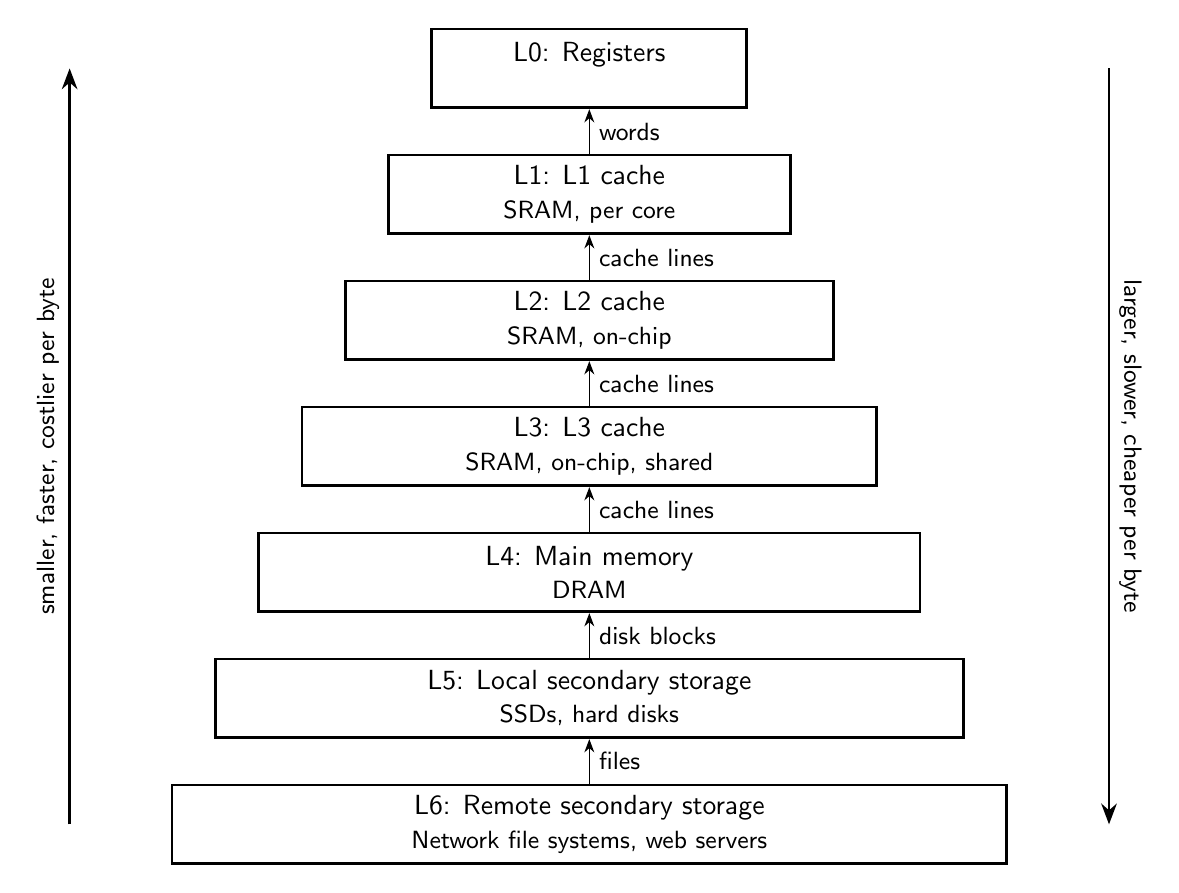
\begin{tikzpicture}[level/.style={draw, align=center, minimum height=1cm}, unit/.style={font=\small, right}]
  % Each level is wider than the one above it: larger, slower, and cheaper per byte.
  \foreach \k/\name/\desc in {0/Registers/{}, 1/L1 cache/{SRAM, per core}, 2/L2 cache/{SRAM, on-chip},
      3/L3 cache/{SRAM, on-chip, shared}, 4/Main memory/DRAM, 5/Local secondary storage/{SSDs, hard disks},
      6/Remote secondary storage/{Network file systems, web servers}}
    \node[level, minimum width=4cm + 1.1cm*\k] (L\k) at (0, -1.6*\k) {L\k: \name \\ {\small \desc}};
  % Each level holds copies of data from the level below, moved in these units.
  \foreach \k/\unit in {1/words, 2/cache lines, 3/cache lines, 4/cache lines, 5/disk blocks, 6/files} {
    \pgfmathtruncatemacro{\above}{\k - 1}
    \draw[->, thin] (L\k.north) -- node[unit] {\unit} (L\above.south);
  }
  \draw[->] (-6.6, -9.6) -- node[sloped, above, font=\small] {smaller, faster, costlier per byte} (-6.6, 0);
  \draw[->] (6.6, 0) -- node[sloped, above, font=\small] {larger, slower, cheaper per byte} (6.6, -9.6);
\end{tikzpicture}
\end{document}
